\documentclass[paper=letter,fontsize=11pt]{scrartcl} % KOMA-article class

\usepackage[english]{babel}
\usepackage[utf8x]{inputenc}
\usepackage[protrusion=true,expansion=true]{microtype}
\usepackage{amsmath,amsfonts,amsthm}     % Math packages
\usepackage{graphicx}                    % Enable pdflatex
\usepackage[svgnames]{xcolor}            % Colors by their 'svgnames'
\usepackage{geometry}
%\textheight=700px                    % Saving trees ;-)
%\usepackage{url}
\usepackage[colorlinks=true,
linkcolor=blue,
urlcolor=blue]{hyperref}
\usepackage{float}
\usepackage{etaremune}
\usepackage{wrapfig}
\usepackage{multicol}

\usepackage{comment}

\usepackage{attachfile}

\frenchspacing              % Better looking spacings after periods
\pagestyle{empty}           % No pagenumbers/headers/footers

%\addtolength{\voffset}{-40pt}
%\addtolength{\textheight}{20pt}

\setlength\topmargin{0pt}
\addtolength\topmargin{-\headheight}
\addtolength\topmargin{-\headsep}
\setlength\oddsidemargin{0pt}
\setlength\textwidth{\paperwidth}
\addtolength\textwidth{-2in}
\setlength\textheight{\paperheight}
%\addtolength\textheight{-3in}
\addtolength\textheight{-2in}
\usepackage{layout}

%%% Custom sectioning}{sectsty package)
%%% ------------------------------------------------------------
\usepackage{sectsty}

\sectionfont{%			            % Change font of \section command
	\usefont{OT1}{phv}{b}{n}%		% bch-b-n: CharterBT-Bold font
	\sectionrule{0pt}{0pt}{-5pt}{1pt}}

%%% Macros
%%% ------------------------------------------------------------
\newlength{\spacebox}
\settowidth{\spacebox}{8888888888}			% Box to align text
\newcommand{\sepspace}{\vspace*{1em}}		% Vertical space macro

\newcommand{\MyName}[1]{ % Name
		\Huge \usefont{OT1}{phv}{b}{n} \hfill #1
		\par \normalsize \normalfont}
		
\newcommand{\MySlogan}[1]{ % Slogan}{optional)
		\large \usefont{OT1}{phv}{m}{n}\hfill \textit{#1}
		\par \normalsize \normalfont}

\newcommand{\NewPart}[2]{\section*{\uppercase{#1} \small \normalfont #2}}

\newcommand{\NewParttwo}[1]{
		\noindent \huge \textbf{#1}
        \normalsize \par}



\newcommand{\PersonalEntry}[2]{\small
		\noindent\hangindent=2em\hangafter=0 % Indentation
		\parbox{\spacebox}{        % Box to align text
		\textit{#1}}		       % Entry name}{birth, address, etc.)
		\small\hspace{1.5em} #2 \par}    % Entry value

\newcommand{\SkillsEntry}[2]{      % Same as \PersonalEntry
		\noindent\hangindent=2em\hangafter=0 % Indentation
		\parbox{\spacebox}{        % Box to align text
		\textsf{#1}}			   % Entry name}{birth, address, etc.)
		\hspace{1.5em} #2 \par}    % Entry value	
		
\newcommand{\EducationEntry}[4]{
		\noindent \textbf{#1} \hfill      % Study
		\colorbox{White}{%
			\parbox{6em}{%
			\hfill\color{Black}#2}} \par  % Duration
		\noindent \textit{#3} \par        % School
		\noindent\hangindent=2em\hangafter=0 \small #4 % Description
		\normalsize \par}

\newcommand{\WorkEntry}[5]{
		\noindent \textbf{#1}
        \noindent \small \textit{#2}
        \hfill      % Study
        \colorbox{White}{%
			\parbox{6em}{%
			\hfill\color{Black}#3}} \par  % Duration
		\noindent \textit{#4} \par        % School
		\noindent\hangindent=2em\hangafter=0 \small #5 % Description
		\normalsize \par}

\newcommand{\Language}[2]{
		\noindent \textbf{#1}
        \noindent \small \textit{#2}}
        
\newcommand{\Text}[1]{\par       
		\noindent \small #1 
		\normalsize \par}
        
\newcommand{\Textlong}[4]{
		\noindent \textbf{#1} \par
        \sepspace
        \noindent \small #2
        \par\sepspace      
		\noindent \small #3
        \par\sepspace      
		\noindent \small #4
        \normalsize \par}
        
\newcommand{\JobSkills}[2]{
		\noindent #1,
		
}
	    
              

\newcommand{\PaperEntry}[7]{
		\noindent #1, ``\href{#7}{#2}", \textit{#3} \textbf{#4}, #5 (#6).}


\newcommand{\ArxivEntry}[3]{
		\noindent #1, ``\href{http://arxiv.org/abs/#3}{#2}", \textit{{cond-mat/}#3}.}
        
\newcommand{\BookEntry}[4]{
		\noindent #1, ``\href{#3}{#4}", \textit{#3}.}
        
\newcommand{\FundingEntry}[5]{
        \noindent #1, ``#2", \$#3 (#4, #5).}

\newcommand{\TalkEntry}[4]{
		\noindent #1, #2, #3 #4}

\newcommand{\ThesisEntry}[5]{
		\noindent #1 -- #2 #3 ``#4" \textit{#5}}

\newcommand{\CourseEntry}[3]{
		\noindent \item{#1: \textbf{#2} \\ #3}}

%%% Begin Document
%%% ------------------------------------------------------------
\begin{document}

%\layout

% you can upload a photo and include it here...
\begin{wrapfigure}{l}{0.5\textwidth}
	\vspace*{-2em}
		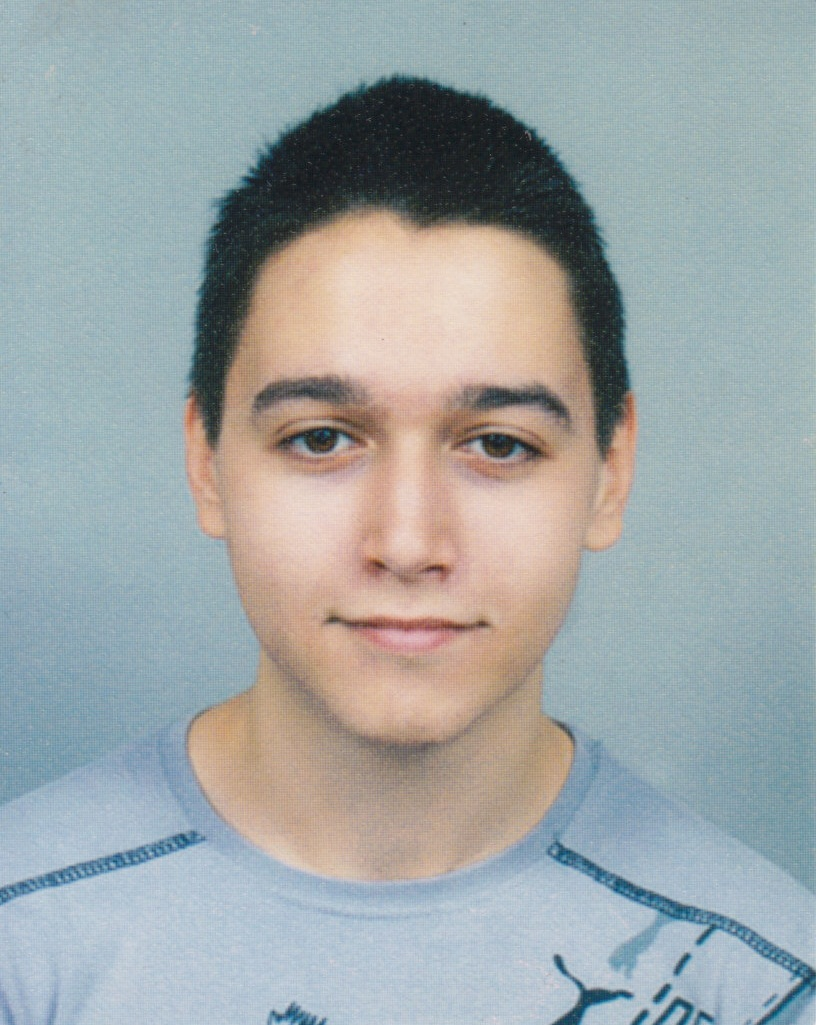
\includegraphics[width=0.15\textwidth]{IMG.jpg}
\end{wrapfigure}

\MyName{Boian Ivanov}
\MySlogan{Curriculum Vit\ae\ } %(\today)}

\sepspace
\sepspace

%%% Personal details
%%% ------------------------------------------------------------
\NewPart{}{}

\begin{multicols}{2}
\PersonalEntry{Address:}{{Lyulin 301}, 1336 Sofia}
\PersonalEntry{Phone:}{+ 359 (0)878448744}
\PersonalEntry{Born:}{27.05.1995}
\PersonalEntry{Nationality:}{Bulgarian, Greek}
\PersonalEntry{Mail:}{\href{mailto:boian.ivanov44@gmail.com}{boian.ivanov44@gmail.com}}
\PersonalEntry{GitHub:}{\href{https://github.com/boian-ivanov/}{github.com/boian-ivanov/}}
\PersonalEntry{LinkedIn:}{\href{https://bg.linkedin.com/in/boianivanov}{linkedin.com/in/BoianIvanov/}}
\PersonalEntry{}{}
\end{multicols}






%%% About Me
%%% ------------------------------------------------------------
\NewPart{About Me}{}
I am a learning programmer in the field of Informatics. My current interest is web programming, but my goal is to be able to code with ease on most available systems. My experience in the field may be limited for now, but my knowledge is ever growing. My passion for my work is what drives me forward in life and my motto is to be the very best, like no one ever was. 

%%% Work experience
%%% ------------------------------------------------------------
\NewPart{Work Experience}{(Reference on demand)}

\WorkEntry{RS Consult}{\href{http://rsc.bg/}{rsc.bg}}{Present}{Sofia, Bulgaria}{Full stack web developer working with PHP, Laravel and OpenCart.}

\sepspace

\WorkEntry{ITR Services}{\href{http://itrservices.eu/}{itrservices.eu}}{2016}{Sofia, Bulgaria}{Web Development Intern. E-commerce development with Magento.}

\begin{comment}
	\item Two months work experience with Wordpress and module development.
	\begin{itemize}
		\item Feza 2017 development, \href{http://feza2017.org/}{feza2017.org}
		\item Co-administration on RSConsult website\href{http://rsc.bg/}{rsc.bg}
	\end{itemize}
	%\item Work experience with Magento module development.
\end{comment}

\sepspace

%%% Education
%%% ------------------------------------------------------------
\NewPart{Education}{}


\EducationEntry{Computer Science and Informatics}
{2013-2017}
{New Bulgarian University, Sofia}
{\begin{itemize}
\item{On-going education in the field of Informatics with focus on Object oriented programming, Web-Programming and Advanced Mathematics}
%\item{}
\end{itemize}}

\sepspace

\EducationEntry{Maintenance of computer systems, applications and networks
}{2011-2013}{Serres, Greece}{
\begin{itemize}\item{Basic knowledge in networking and programming}\end{itemize}}

\begin{comment}
%%% Job Qualifications
%%% ------------------------------------------------------------
\NewPart{Job Qualifications}{}
\sepspace
\begin{description}
\item[]{Skilled at Front and Back-end programming with HTML, CSS, XML and PHP.}
\item[]{Good database and SQL knowledge.}
\item[]{Programming in OOP languages.}
\item[]{Capable of working under either Windows or Linux OS (Ubuntu, Mint, Debian, CentOS).}
\end{description}

%\SkillsEntry{Programing}{Java, C++, Html}




%%% Work experience
%%% ------------------------------------------------------------
\NewPart{Work Experience}{(Reference on demand)}

\WorkEntry{Expoprojekt}{\href{http://expoprojekt.se}{expoprojekt.se}}{2015}{Stockholm, Sweden}{Exhibition production manager. Part-time during the whole year and different projects during summer.}

\sepspace

\WorkEntry{Jernhusen}{\href{http://jernhusen.se}{jernhusen.se}}{2014}{Stockholm, Sweden}{Organization during summer of a computer system for real estate energy. Jernhusen owns main part of the real estate connected to the Swedish railway.}

\sepspace

\WorkEntry{Alpingaraget, alpint AB}{\href{http://alpingaraget.se}{alpingaraget.se}}{2012-2015}{Stockholm, Sweden}{Part-time sales of sport goods, (mainly skis), ski service and customer service.}
\newpage

\WorkEntry{Sandgren Electronics AB}{\href{http://iphonereparation.se}{iphonereparation.se}}{2012-2013}{Gothenburg/ Stockholm, Sweden}{Summer vacation work experience and part-time. Electronic repairs, mainly cell phones.}

\sepspace

\WorkEntry{Active Ski Travel Scandinavia AB}{\href{http://www.activeski.se}{activeski.se}}{2012}{Engelberg, Switzerland}{Travel guide during winter. Responsible for guests traveling to Engelberg.}

\sepspace

\WorkEntry{Surefoot}{\href{http://www.surefoot.com}{surefoot.com}}{2011}{Verbier, Switzerland}{Part-time winter. Building custom-made ski boots. Sales of sport goods, mainly ski boots.}
\sepspace

\WorkEntry{M?ssmix Design AB }{}{2009-2013}{Stockholm, Sweden}{Fulltime employee as exhibition production manager 2009. Part-time during different projects until 2013. Work-tasks: Planning, designing and manufacturing exhibitions-stands to different exhibitions through out the world.}
\sepspace

\WorkEntry{Bj?rk and S?derqvist construction AB}{\href{http://bjorksoderqvist.com}{bjorksoderqvist.com}}{2008-2009}{Stockholm, Sweden}{Carpenter at Bj?rk and S?derqvist during Fall 2008 and summer 2009.}

\sepspace


%%% OTHER QUALIFICATIONS
%%% ------------------------------------------------------------
\NewPart{OTHER QUALIFICATIONS}{}

\WorkEntry{Founding and developing a ski-company, Skadi skis}{\href{https://www.facebook.com/skadiskis/}{Skadiskis.se}}{2008-2013}{Stockholm, Sweden}{Production of a pair of alpine skis during the last year of upper secondary school with a friend, which later on resulted in the founding of Skadi skis.

\sepspace

\WorkEntry{Snow safety education, 8 days}{\href{http://www.strapatser.se}{strapatser.se}}{2006}{Fun?sdalen, Sweden}{Education with focus on avalanche and ski safety.}
\sepspace
\end{comment}

%%% LANGUAGES
%%% ------------------------------------------------------------
\NewPart{LANGUAGES}{}

\Language{Bulgarian}{(mother tongue),}
\Language{Greek}{ (fluent),}
\Language{English}{(fluent),}
\Language{German}{(B1)}


\begin{comment}
\NewPart{OTHER QUALIFICATIONS}{}

\WorkEntry{Drivers license}{}{2015}{Sofia, Bulgaria}{Car (B,B1) and Motorbike(AM)}



\begin{comment}
\NewPart{Interests and personality}{}

\Text{Traveling is a big part of my life. I enjoy going to new places and meeting new people, while exploring the world, piece by piece at a time. My friends and family form my other big interest. I see myself as a happy, outgoing and reliable person. I am a problem solver and no challenge is too big. The result of my work is often better than expected.}
\newpage


%%% Letter
%%% ------------------------------------------------------------

\NewParttwo{Anschreiben V?lkl}

\sepspace



\Textlong{Praktikant im bereich entwicklung/labor ski/snowboard.}{Sehr geehrte(r) herr oder frau}{Mein Name ist Mikael Kajbring. Ich bin 26 Jahre alt und komme aus Stockholm. Ich wohne in M?nchen und bin ein Erasmus-Student an der Technischen Universit?t M?nchen (TUM). Ich studiere Maschinenbau/ Fahrzeugtechnik im dritten Jahr mit Ausrichtung Management. Nach dem Abitur an einer technischen Schule habe ich eine Ski-Firma (Skadi-skis) gegr?ndet, in der ich Freerideski f?r den schwedischen und schweizer Markt angefertigt habe. Die Firma gibt es jetzt nicht mehr, aber ich entwickle weiter Ski f?r mich und Freunde. Ich habe mit vielen Materialien gearbeitet wie Titanal, Polyurethan, Kohlefaser und Bambus. Weil die Firma nicht gro? war, habe ich Produktion, Marketing und Vertrieb geleitet. Ich habe auch Fertigkeiten mit CAD- und Graphikdesign-Programmen, weil ich alle Entw?rfe und Topsheets selbst gemacht habe. W?hrend meines Studiums habe ich auch in einem kleinen Skigesch?ft in Stockholm gearbeitet. 
Meine Leidenschaften sind Skifahren und das Leben in der Natur. Zwischen 2010 und 2014 habe ich an Wettk?mpfen der Freeride World Qualifier teilgenommen und ich habe viele Freunde in der Freeride World Tour, unter anderem euren Fahrer Sam Smoothy. 
Ich sehe mich selbst als einen gl?cklichen und sympathischen Menschen. Meine englischen Sprachkenntnisse sind sehr gut und durch das Erlernen der deutschen Sprache hoffe ich meine sozialen F?higkeiten zu erweitern. Nach dem Studium will ich in der Entwicklung von Sportger?ten arbeiten und ich hoffe, ich kann bei V?lkl damit anfangen.
Mit diesem Hintergrund m?chte ich fragen, ob Sie f?r mich eine Praktikumstelle im n?chsten Jahr haben.}{Mit freundlichen Gr??en, Mikael Kajbring}

\sepspace

%\begin{wrapfigure}{l}{\textwidth}
%		\vspace{5em}
%        \centering
%		\includegraphics[height=0.25\textwidth]{IMG_0068.JPG}
%        \hspace{1em}
%        \includegraphics[height=0.25\textwidth]{154327_165817636790533_1488132_n.jpg}
        
%\end{wrapfigure}

%\begin{wrapfigure}{l}{\textwidth}
%		\vspace{1em}
%        \centering            
%        \includegraphics[height=0.25\textwidth]{133107_166579826714314_3462381_o.jpg}
%        
%\end{wrapfigure}




https://www.overleaf.com/articles/kajbring-cv/bsvjnmqwxrqd#.Vv1q6tJ96M8
\end{comment}


\end{document}
